\stepcounter{footnote}\newcounter{pizzachili}\setcounter{pizzachili}{\value{footnote}}
\stepcounter{footnote}\newcounter{xmldata}\setcounter{xmldata}{\value{footnote}}

\begin{table}[H]
\centering
\makebox[0pt][c]{\parbox{1.0\textwidth}{%
    \begin{minipage}[b]{0.48\hsize}\centering
      \begin{tabular}{c|rrrrr}
       $p$ & {\tt wiki} & {\tt prot} & {\tt dna} & {\tt ctree} & {\tt osm}\\
       %   $(n)$ & (498,753,915) & (670,721,005) & (1,154,482,174) & (2,147,483,644) & (4,675,776,358)\\
        \hline
        \hline
        1 & 2.89 & 4.22 & 7.21 & 12.16 & 30.60 \\
        4 &  .73 & 1.10 & 1.87 & 3.18 & 7.98 \\
        8 &  .37 &  .57 &  .98 & 1.59 & 4.14 \\
        12 &  .31 &  .44 &  .72 & 1.15 & 3.07 \\
        16 &  .25 &  .35 &  .58 &  .86 & 2.21 \\
        20 &  .23 &  .32 &  .55 &  .76 & 1.83 \\
        24 &  .21 &  .28 &  .46 &  .69 & 1.72 \\
        28 &  .18 &  .28 &  .45 &  .63 & 1.55 \\
        32 &  .18 &  .25 &  .39 &  .63 & 1.33 \\
        36 &  .16 &  .25 &  .39 &  .55 & 1.33 \\
        40 &  .18 &  .26 &  .35 &  .51 & 1.27 \\
        44 &  .17 &  .27 &  .35 &  .49 & 1.14 \\
        48 &  .22 &  .28 &  .38 &  .53 & 1.21 \\
        52 &  .24 &  .26 &  .33 &  .46 & 1.09 \\
        56 &  .21 &  .28 &  .39 &  .49 & 1.02 \\
        60 &  .28 &  .29 &  .39 &  .46 & 1.04 \\
        64 &  .27 &  .29 &  .39 &  .48 & 1.01 \\
         \hline
      \end{tabular}
      \caption{Running times (seconds) {\tt PSTA} on different data sets, using 1 up to 64 processors.}
%%\caption[]{Relative speed-up achieved on different data sets using our {\tt PSTA}
%%  algorithm compared to {\tt PSTA} on a single processor, {\tt libcds}, and {\tt
%%    sdsl}, respectively.
%%  The latter two are sequential algorithms.
%%  This speed-up is the running time of the respective comparator algorithm
%%  divided by the running time of {\tt PSTA} on the number of processors listed
%%  in the leftmost column.
%%  The data sets were LZ78 parsings of the XML ({\tt xml}), DNA ({\tt dna}), and
%%  protein ({\tt protein}) data from the Pizza \& Chili
%%  corpus\footnotemark[\value{pizzachili}], as well as data from the XMLData
%%  repository\footnotemark[\value{xmldata}] ({\tt psd7003}) and a complete binary tree of
%%  depth 30 ({\tt comptree}).
%%  The number of parentheses in the input, which is twice the number of nodes in
%%  the tree, is listed in parentheses for each data set.}
      \label{tbl:parallelTimes}
    \end{minipage}
    \hfill
    \begin{minipage}[b]{0.48\hsize}\centering
      \begin{tabular}{c|rrrrr}
        & {\tt wiki} & {\tt prot} & {\tt dna} & {\tt ctree} & {\tt osm}\\
        \hline
        \hline
        {\tt libcds} & 33.12 & 44.16 & 75.81 & 140.97 & 26.97 \\
        {\tt sdsl} & 1.93 & 2.66 & 4.57 & 8.35 & 18.10 \\
        \hline
      \end{tabular}
      \caption{Running times (seconds) of state-of-the-art implementations {\tt libcds} and {\tt sdsl}.}
      \label{tbl:sequetialTimes}

      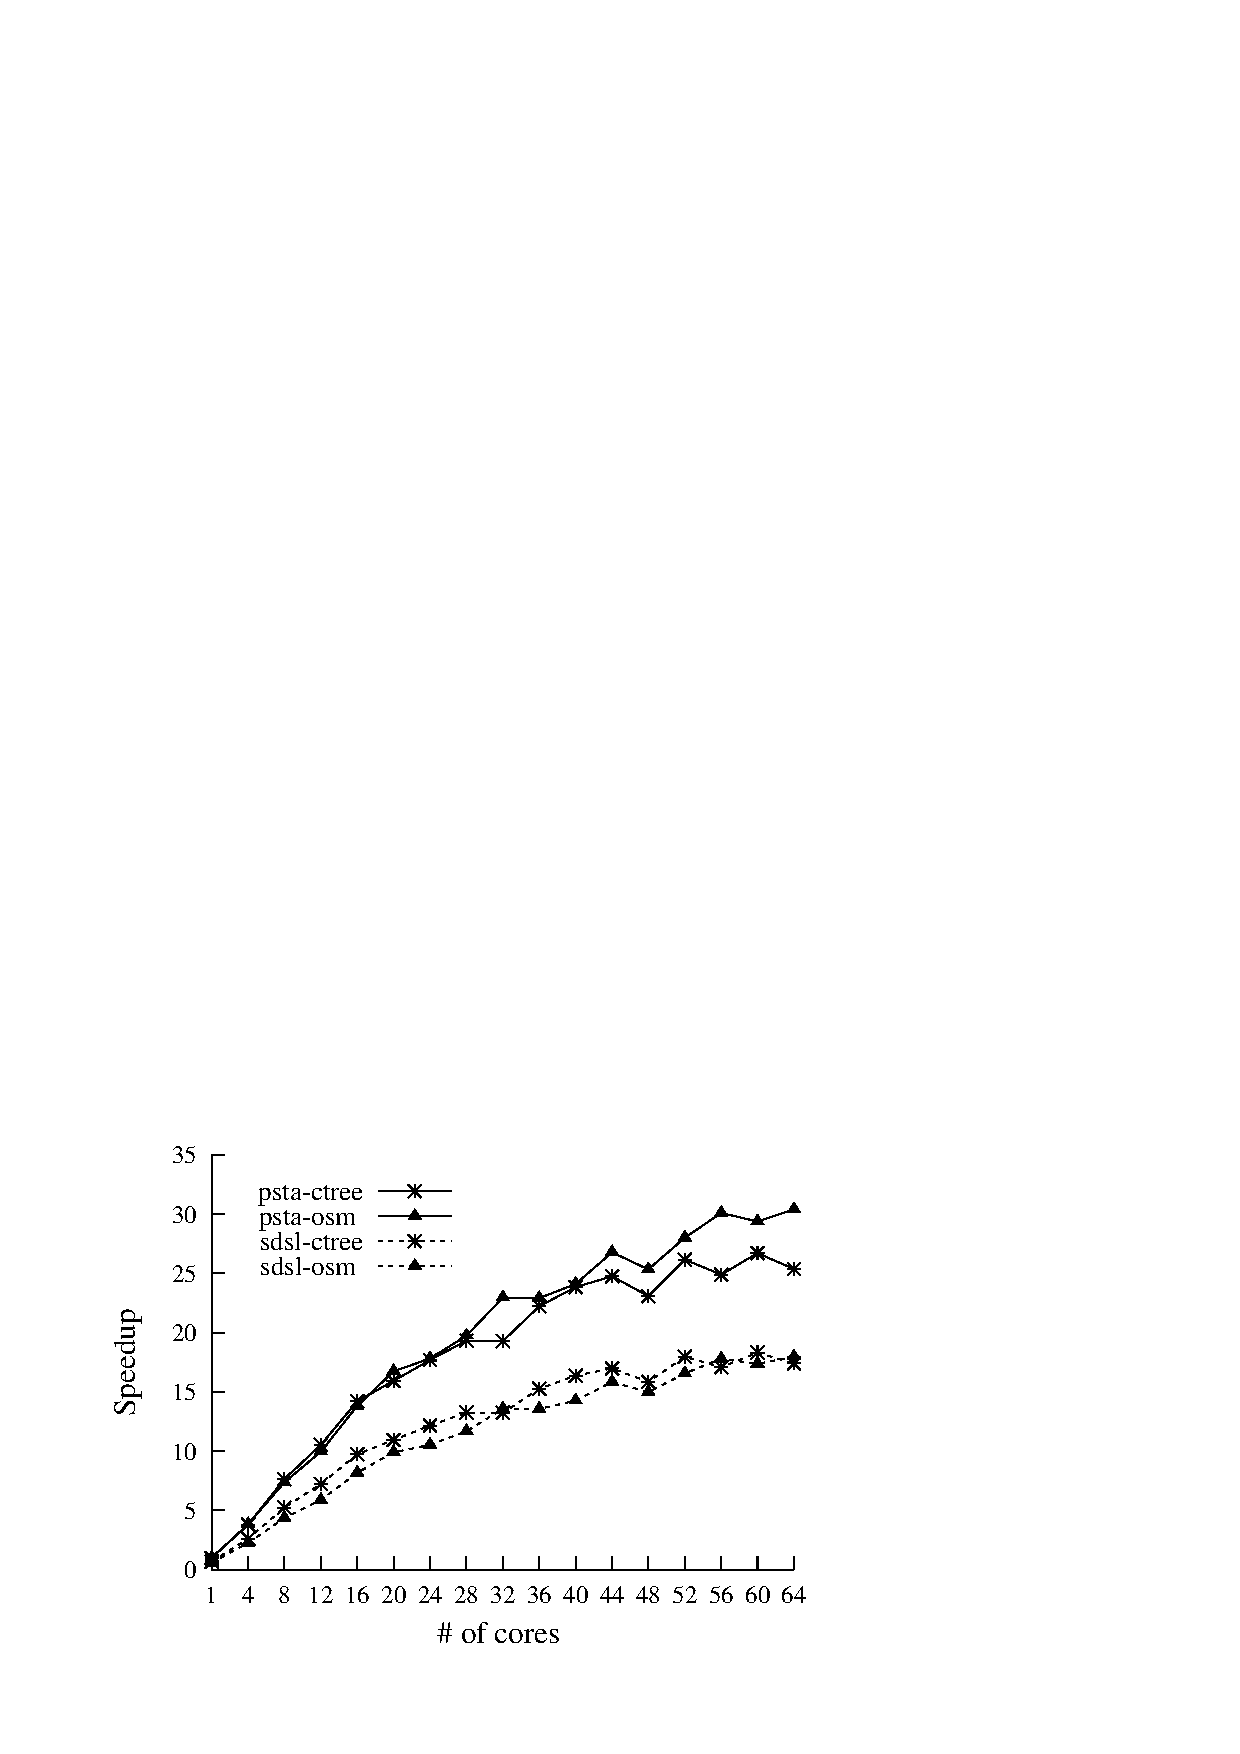
\includegraphics[scale=0.5]{./images/speedup}
      \caption{Relative speed-up achieved on {\tt Comptree} and {\tt Open Street Map} data sets.}
      \label{fig:speedup}

    \end{minipage}
}}
\end{table}


Table~\ref{tbl:speedup} shows the wall-clock time results obtained by
our {\tt psta} algorithm compared to \verb+libcds+ and \verb+sdls+.
We repeated each experiment three times and recorded the minimum
running time, assuming that slightly larger values of any given
experiment are just ``noise'' from external processes such as
operating system and networking tasks.\Norbert{One can often argue
  that the opposite is the case: When the cache is already primed, you
  often see better performance than on an unprimed cache.  So the
  right way of doing this is to run each experiment 3 times, but not 3
  times in a row, to avoid cache priming.}


First note that {\tt psta} outperformed {\tt libcds} by an order of
magnitude even on a single core. There are two reasons for this:
first, \verb+libcds+ implements a different version of \verb+RMMT+
whereby it builds {\em rank} and {\em select} structures, while
\verb+psta+ and \verb+sdsl+ do not\footnote{They are actually not part
  of the original proposal by
  \cite{Navarro:2014:FFS:2620785.2601073}.}. This makes the whole
process costlier. Second, as we allowed {\tt psta} to utilize more
cores, its advantage over {\tt libcds} only increased because {\tt
  libcds} is a purely sequential program.  {\tt sdsl} was about 1.5
times faster than {\tt psta} on a single core, but already using two
cores {\tt psta} started to be faster than {\tt sdsl}, again because
{\tt sdsl} is a purely sequential program.  The advantage of {\tt
  sdsl} over {\tt psta} on a single core, in spite of implementing
essentially the same algorithm, can be attributed to (1) lack of
tuning of {\tt psta} and (2) some overhead with running parallel code
on a single core, which {\tt sdsl} avoids by being a purely sequential
program.

Up to 16 cores, the speed-up is almost linear whenever $p$ is a power
of $2$, with an efficiency of 60\%, which is quite good for multicore
architectures.  When $p$ is not a power of $2$, speed-up is slightly
worse.  The reason is that, when $p$ is a power of $2$, {\tt psta} can
assign exactly one subtree per thread (see Algorithm
\ref{algo:PSTA2}), distributing the work homogeneously across cores
and thus not requiring any work stealing.  When the number of threads
is not a power of two, some threads have to process more than one
subtree and other threads process only one, which degrades
performance.  Nevertheless, due to work stealing, no core sits idle
for long and the slight performance degradation is due to the overhead
of work stealing.\Norbert{I made this up.  Does this make sense?
  Essentially, the way it was phrased before doesn't really offer a
  lot of insight into where the performance degradation really comes
  from when the work is not distributed evenly, and what I wrote here
  at least matches that we point out that no work stealing is required
  when $p = 2^x$.}  For $p = 32$, the efficiency of {\tt psta} drops
below 50\%.  This is likely because, on our 32-core machine, less than
32 threads can execute on their own dedicated cores without
interfering with OS processes, which can run on the 32nd core.  When
using 32 threads, the threads of our program start to compete with OS
processes for the available cores, which degrades performance.

The general performance degradation beyond 16 threads is most likely
due to the architecture of the machine we ran our experiments on.  The
4 processors on this machine are arranged in a grid
topology~\cite{Drepper2007}.  Up to 8 threads, communication between
the threads is limited to a single processor running these threads,
with very little overhead.  Between 8 and 16 threads require the use
of two adjacent processors in the grid, which still keeps
communication cost low.  Beyond 16 threads, three or four processors
are needed and at least two of these processors are not adjacent in
the grid, which increases the communication between the threads on
these processors noticeably.  \Leo{Review Drepper's explanation of
  this}.

Since {\tt psta} generates tasks that work on different memory
regions, the generated cache misses \Leo{false sharing is misses} do
not degrade the performance. The same effect is present on
\emph{Domain Decomposition Algorithms}. Although the decomposition of
the {\tt RMMT} was not evident, we could produce a decomposition that
generated a competitive algorithm.\Norbert{I'm not sure what exactly
you're saying here.  Are you saying that, if the threads were working on the
same memory regions, maintaining cache coherence would essentially force
a lot of reads from RAM because pages in cache become invalid due to writes
by other processors, and given that all our threads work on different memory
regions, this issue does not arise?}
%	
%\begin{table}[ht]
%  \centering
%  \begin{tabular}{crrrrr}
%\hline
%    & xml & dna & psd7003 & protein & comptree\\
%\hline
% \verb|psta|   &  1.46  &  1.74  & 2.78  &  3.30 & 112.01\\
% \verb|libcds|   &  .42 &  .58 & .77 &  1.08 & 38.25\\
% \verb|sdsl|   &  .95 &  1.31 & 1.73 &  2.41 & 76.40\\
% \hline
%\end{tabular}
%\caption{Peak memory consumption of the three algorithms on the data sets
%  from Table~\ref{tbl:speedup}, measured in MB.}
%\label{tbl:memory_consumption}
%\end{table}

Table \ref{tbl:memory_consumption} shows memory consumption for the
corpora usid in our experiments.  For {\tt psta}, the consumption of
the single-threaded code ($p = 1$) is shown.  The extra memory needed
for thread scheduling when $p > 1$ was negligible.  To measure memory
consumption, we monitored how much memory was allocated with
\texttt{malloc} and released with \texttt{free} at execution time and
recorded the peak consumption.  We only measured memory allocated
during construction of the data structure, which does not include the
memory allocated to store the parenthesis sequence.  Even though {\tt
  psta} consumes more memory than both {\tt libcds} and {\tt sdsl},
the difference between {\tt psta} and {\tt sdsl} is a factor of less
than two.  The difference between {\tt psta} and {\tt libcds} is no
more than a factor of four and is outweighed by the substantially
worse performance of {\tt libcds}, even compared to the
single-threaded version of {\tt psta}.  More importantly, a memory
consumption of 112MB for processing a 1-billion-node tree amounts to
less than one bit per node and, so {\tt psta} can be considered very
space-efficient.

\footnotetext[\value{pizzachili}]{\url{http://pizzachili.dcc.uchile.cl}}
\footnotetext[\value{xmldata}]{\url{http://www.cs.washington.edu/research/xmldatasets}}

Part of the higher memory consumption of {\tt psta} compared to {\tt
  libcds} and {\tt sdsl} stems from the allocation of $e^{\prime}$,
$m^{\prime}$, $M^{\prime}$ and $n^{\prime}$ arrays to store the
partial excess values in the algorithm.  Storing these values is a key
factor that helps {\tt psta} to achieve very good performance.  Our
implementation allocates 16 bits per excess value in these arrays.  It
would be possible to use a simplification of Algorithm
\ref{algo:PSTA1} to calculate the depth $d$ of the input sequence (the
maximum excess value) and then allocate only $\lg d$ bits per excess
value to reduce the space overhead of storing these areas and improve
performance further by reducing the memory bandwidth required to read
and write these arrays.

%\begin{table*}[ht]
%  \centering
%  \begin{tabular}{crrrrrrrrrrrrrrr}
%    \hline
%    p & XML  & DNA  & psd7003 & Proteins & Concat & CompTree \\
%    \hline
%    1       & 0.60 & 0.64 & 0.63    & 0.61     & 0.62   & 0.69     \\
%    4       & 2.30 & 2.48 & 2.41    & 2.41     & 2.43   & 2.62     \\
%    8       & 4.36 & 4.67 & 4.21    & 4.60     & 4.55   & 5.24     \\
%    12      & 4.63 & 5.01 & 4.87    & 5.88     & 6.31   & 7.23     \\
%    16      & 4.32 & 5.38 & 4.59    & 5.21     & 6.51   & 9.74     \\
%    20      & 4.38 & 5.38 & 5.07    & 7.29     & 7.66   & 10.93    \\
%    24      & 3.51 & 4.58 & 5.69    & 5.98     & 6.03   & 12.13    \\
%    28      & 2.73 & 3.71 & 3.42    & 4.02     & 6.90   & 13.24    \\
%    32      & 2.14 & 3.24 & 4.03    & 3.58     & 7.01   & 13.22    \\
%    36      & 4.16 & 6.29 & 2.59    & 4.73     & 5.72   & 15.23    \\
%    40      & 1.63 & 3.11 & 4.09    & 3.96     & 5.19   & 16.34    \\
%    44      & 1.98 & 2.07 & 3.36    & 3.23     & 4.60   & 16.97    \\
%    48      & 1.15 & 2.85 & 2.33    & 3.60     & 5.60   & 15.82    \\
%    52      & 1.30 & 1.82 & 1.78    & 2.31     & 5.01   & 17.94    \\
%    56      & 1.01 & 1.35 & 2.13    & 3.10     & 3.54   & 17.07    \\
%    60      & 1.03 & 1.67 & 1.59    & 1.85     & 3.82   & 18.30    \\
%    64      & 1.34 & 1.44 & 2.11    & 2.58     & 2.68   & 17.39    \\
%    \hline\hline
%\end{tabular}
%\caption{Speedup of {\tt psta} over the state-of-the-art implementation {\tt sdls}}
%\label{tbl:speedup}
%\end{table*}
